\documentclass{article}\usepackage[]{graphicx}\usepackage[]{color}
%% maxwidth is the original width if it is less than linewidth
%% otherwise use linewidth (to make sure the graphics do not exceed the margin)
\makeatletter
\def\maxwidth{ %
  \ifdim\Gin@nat@width>\linewidth
    \linewidth
  \else
    \Gin@nat@width
  \fi
}
\makeatother

\definecolor{fgcolor}{rgb}{0.345, 0.345, 0.345}
\newcommand{\hlnum}[1]{\textcolor[rgb]{0.686,0.059,0.569}{#1}}%
\newcommand{\hlstr}[1]{\textcolor[rgb]{0.192,0.494,0.8}{#1}}%
\newcommand{\hlcom}[1]{\textcolor[rgb]{0.678,0.584,0.686}{\textit{#1}}}%
\newcommand{\hlopt}[1]{\textcolor[rgb]{0,0,0}{#1}}%
\newcommand{\hlstd}[1]{\textcolor[rgb]{0.345,0.345,0.345}{#1}}%
\newcommand{\hlkwa}[1]{\textcolor[rgb]{0.161,0.373,0.58}{\textbf{#1}}}%
\newcommand{\hlkwb}[1]{\textcolor[rgb]{0.69,0.353,0.396}{#1}}%
\newcommand{\hlkwc}[1]{\textcolor[rgb]{0.333,0.667,0.333}{#1}}%
\newcommand{\hlkwd}[1]{\textcolor[rgb]{0.737,0.353,0.396}{\textbf{#1}}}%

\usepackage{framed}
\makeatletter
\newenvironment{kframe}{%
 \def\at@end@of@kframe{}%
 \ifinner\ifhmode%
  \def\at@end@of@kframe{\end{minipage}}%
  \begin{minipage}{\columnwidth}%
 \fi\fi%
 \def\FrameCommand##1{\hskip\@totalleftmargin \hskip-\fboxsep
 \colorbox{shadecolor}{##1}\hskip-\fboxsep
     % There is no \\@totalrightmargin, so:
     \hskip-\linewidth \hskip-\@totalleftmargin \hskip\columnwidth}%
 \MakeFramed {\advance\hsize-\width
   \@totalleftmargin\z@ \linewidth\hsize
   \@setminipage}}%
 {\par\unskip\endMakeFramed%
 \at@end@of@kframe}
\makeatother

\definecolor{shadecolor}{rgb}{.97, .97, .97}
\definecolor{messagecolor}{rgb}{0, 0, 0}
\definecolor{warningcolor}{rgb}{1, 0, 1}
\definecolor{errorcolor}{rgb}{1, 0, 0}
\newenvironment{knitrout}{}{} % an empty environment to be redefined in TeX

\usepackage{alltt}
\usepackage{amsmath}
\usepackage{amssymb}
\IfFileExists{upquote.sty}{\usepackage{upquote}}{}
\begin{document}



\title{STAT215A - Redwood Data Lab}
\author{Timothy Meyers}
\maketitle



Exploration of Data

Please read the paper to understand how the sensor works, and write a paragraph to discuss the measurement of each variable you 􏰃nd interesting in the data. Please have at least 3 variables in your report, and those variables should be related to your 􏰃ndings in 1.3.

1) Variables

The data is measured from a series of sensors which collect temperature, humidity, and luminosity readings.  The Sensirion SHT11 is a digital sensor that records both temperature and humidity.  The measurement error for each of these variables is ± 0.5◦C and ± 3.5 percent, respectively.  Humidity is greater than zero, but can be greater than 100 percent in foggy conditions. Temperature readings, even if they are within normal ranges, can deviate significantly from historical values depending on the sensor's battery.  Voltage is recorded and provides an indication of the reliability of temperature recordings, and it's advised to focus only on temperature readings generated from a sensor with voltage between 2.4 and 3.  Luminosity is recorded as Photosynthetically active radiation (PAR), and both incident (direct) and reflected (ambient) PAR are recorded.  These measurements are collected by two Mamamatsu S1087 photodiodes, and are referred to as hamatop and hamabot in the data.  The units of measurement are unclear.

2) Data Cleaning

Bearing the data quality in mind, your second task will be data cleaning. This data set is quite raw - it contains some gross outliers, inconsistencies, and lots of missing values. Read the 􏰅Outlier rejection􏰆 section in the paper carefully and critically. You will need to do some cleaning of the data but don't blindly follow their method. Record in your report the steps you take and any evidence you use to support them.

After loading the data and making a few plots, I saw that some rows had values missing.  Also, looking at the plots helped me understand the ranges where values were expected to lie, allowing me to remove obvious outliers.



\ref{fig:plot_raw_humid_temp}.

\begin{knitrout}
\definecolor{shadecolor}{rgb}{0.969, 0.969, 0.969}\color{fgcolor}\begin{figure}[h!]


{\centering 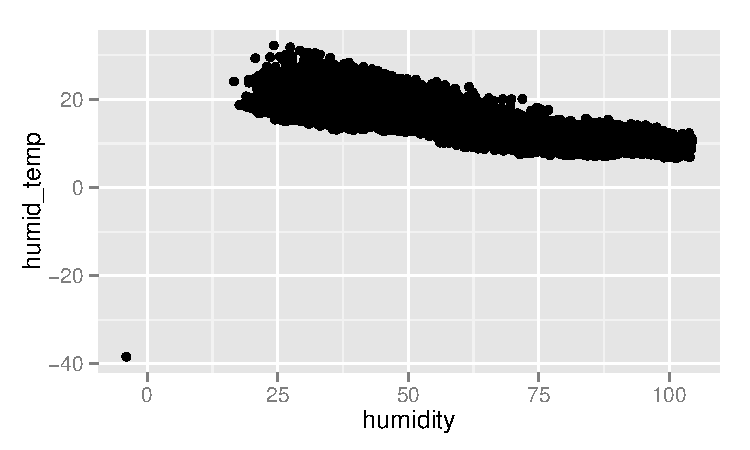
\includegraphics[width=\maxwidth]{figure/plot_raw_humid_temp} 

}

\caption[Observe expected range for humidity and humidtemp]{Observe expected range for humidity and humidtemp\label{fig:plot_raw_humid_temp}}
\end{figure}


\end{knitrout}

\ref{fig:plot_cleansed_humid_temp}.
\begin{knitrout}
\definecolor{shadecolor}{rgb}{0.969, 0.969, 0.969}\color{fgcolor}\begin{figure}[h!]


{\centering 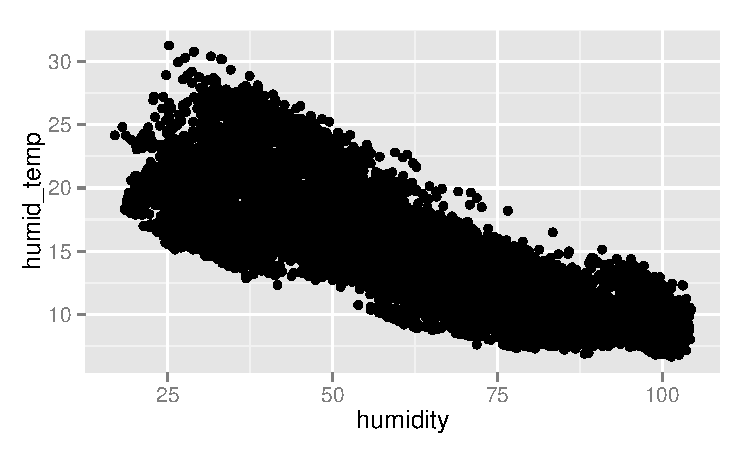
\includegraphics[width=\maxwidth]{figure/plot_cleansed_humid_temp} 

}

\caption[Remove empty values and outliers (humidtemp and humidity)]{Remove empty values and outliers (humidtemp and humidity)\label{fig:plot_cleansed_humid_temp}}
\end{figure}


\end{knitrout}

\ref{fig:plot_raw_hama}.
\begin{knitrout}
\definecolor{shadecolor}{rgb}{0.969, 0.969, 0.969}\color{fgcolor}\begin{figure}[h!]


{\centering 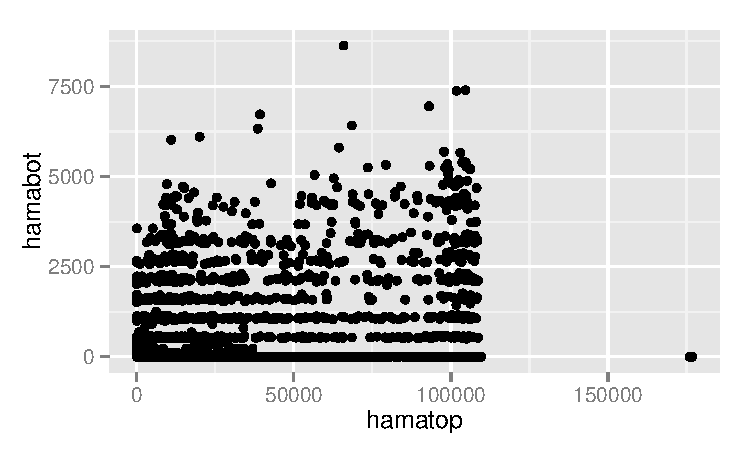
\includegraphics[width=\maxwidth]{figure/plot_raw_hama} 

}

\caption[Observe expected range for hamatop and hamabot]{Observe expected range for hamatop and hamabot\label{fig:plot_raw_hama}}
\end{figure}


\end{knitrout}

\ref{fig:plot_cleansed_hama}.
\begin{knitrout}
\definecolor{shadecolor}{rgb}{0.969, 0.969, 0.969}\color{fgcolor}\begin{figure}[h!]


{\centering 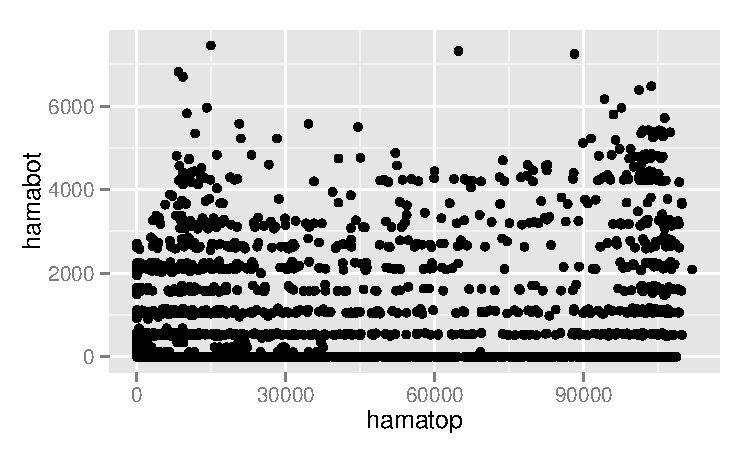
\includegraphics[width=\maxwidth]{figure/plot_cleansed_hama} 

}

\caption[Remove empty values and outliers (Hamatop and Hamabot)]{Remove empty values and outliers (Hamatop and Hamabot)\label{fig:plot_cleansed_hama}}
\end{figure}


\end{knitrout}

\ref{fig:plot_raw_voltage_humidity}
\begin{knitrout}
\definecolor{shadecolor}{rgb}{0.969, 0.969, 0.969}\color{fgcolor}\begin{figure}[h!]


{\centering 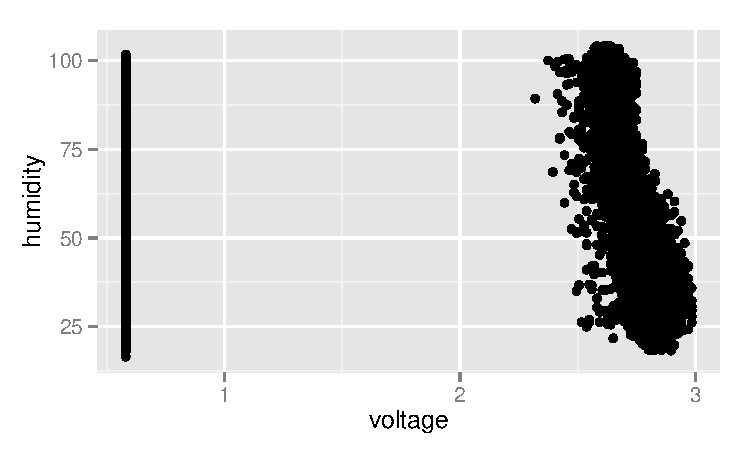
\includegraphics[width=\maxwidth]{figure/plot_raw_voltage_humidity} 

}

\caption[Observe expected range for voltage and humidity]{Observe expected range for voltage and humidity\label{fig:plot_raw_voltage_humidity}}
\end{figure}


\end{knitrout}

\ref{fig:plot_cleansed_voltage_humidity}
\begin{knitrout}
\definecolor{shadecolor}{rgb}{0.969, 0.969, 0.969}\color{fgcolor}\begin{figure}[h!]


{\centering 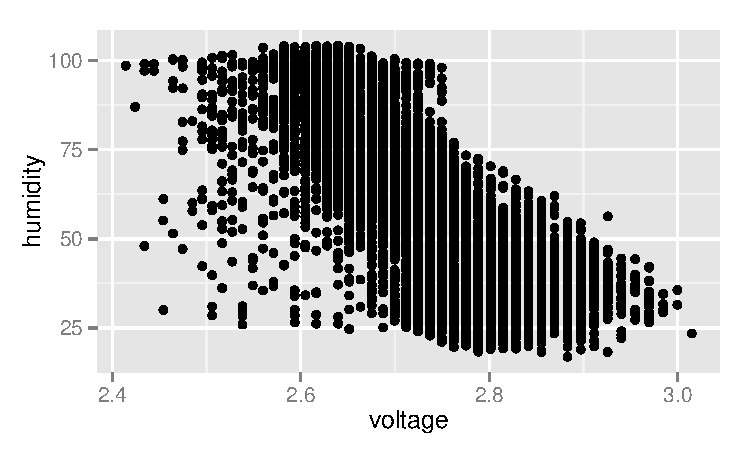
\includegraphics[width=\maxwidth]{figure/plot_cleansed_voltage_humidity} 

}

\caption[Remove empty values and outliers (voltage)]{Remove empty values and outliers (voltage)\label{fig:plot_cleansed_voltage_humidity}}
\end{figure}


\end{knitrout}

After applying basic data cleansing to the net and log data, I ran humidity and temperature versus epoch on the net data and found that there were quite a few outliers in the temperature measurements.  These became more apparent when plotting against voltage, and I decided that 240 was the appropriate voltage cutoff to remove these outliers.

\ref{fig:plot_raw_net_epoch_humidity}

\begin{knitrout}
\definecolor{shadecolor}{rgb}{0.969, 0.969, 0.969}\color{fgcolor}\begin{figure}[h!]


{\centering 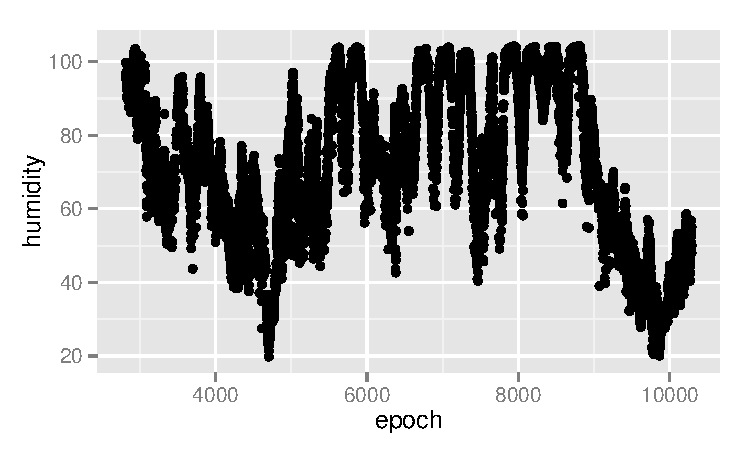
\includegraphics[width=\maxwidth]{figure/plot_raw_net_epoch_humidity} 

}

\caption[Observe humidity over time]{Observe humidity over time\label{fig:plot_raw_net_epoch_humidity}}
\end{figure}


\end{knitrout}

\ref{fig:plot_raw_net_epoch_humid_temperature}
\begin{knitrout}
\definecolor{shadecolor}{rgb}{0.969, 0.969, 0.969}\color{fgcolor}\begin{figure}[h!]


{\centering 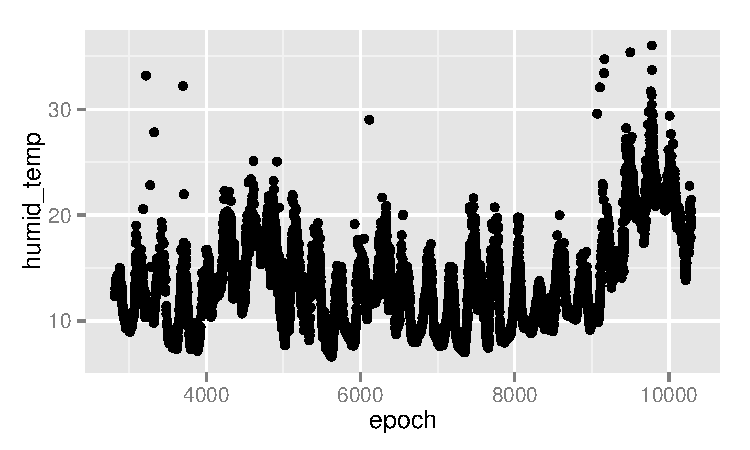
\includegraphics[width=\maxwidth]{figure/plot_raw_net_epoch_humid_temperature} 

}

\caption[Observe temperature over time]{Observe temperature over time\label{fig:plot_raw_net_epoch_humid_temperature}}
\end{figure}


\end{knitrout}

\ref{fig:plot_raw_net_voltage_temperature}
\begin{knitrout}
\definecolor{shadecolor}{rgb}{0.969, 0.969, 0.969}\color{fgcolor}\begin{figure}[h!]


{\centering 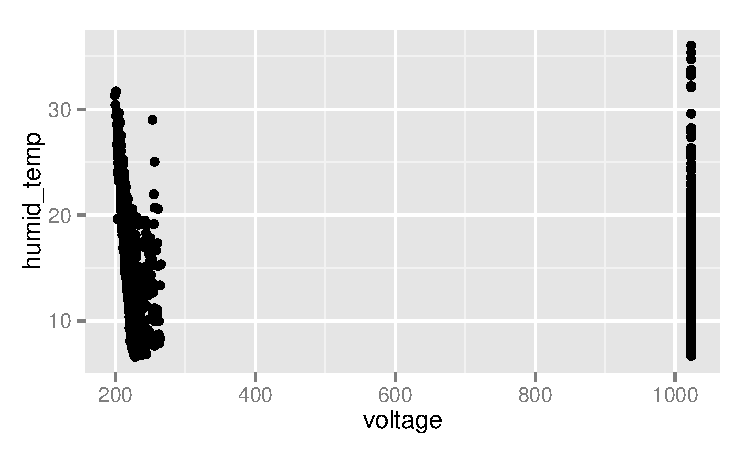
\includegraphics[width=\maxwidth]{figure/plot_raw_net_voltage_temperature} 

}

\caption[Observe temperature over voltage]{Observe temperature over voltage\label{fig:plot_raw_net_voltage_temperature}}
\end{figure}


\end{knitrout}

\ref{fig:plot_cleansed_net_voltage_temperature}
\begin{knitrout}
\definecolor{shadecolor}{rgb}{0.969, 0.969, 0.969}\color{fgcolor}\begin{figure}[h!]


{\centering 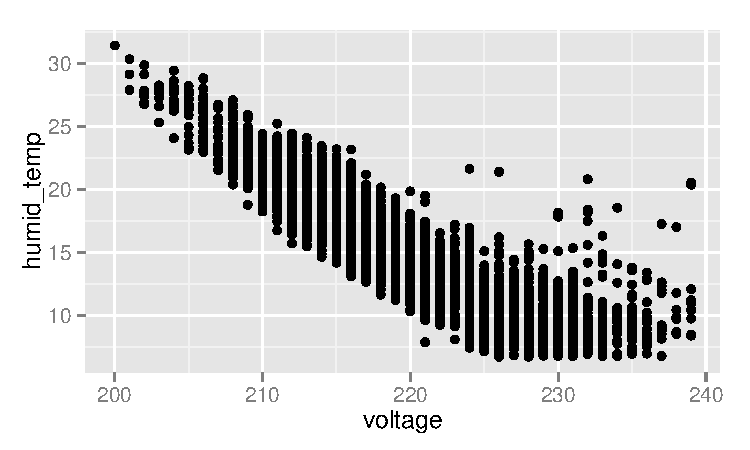
\includegraphics[width=\maxwidth]{figure/plot_cleansed_net_voltage_temperature} 

}

\caption[Remove voltage outliers]{Remove voltage outliers\label{fig:plot_cleansed_net_voltage_temperature}}
\end{figure}


\end{knitrout}

\ref{fig:plot_cleansed_net_epoch_temperature}
\begin{knitrout}
\definecolor{shadecolor}{rgb}{0.969, 0.969, 0.969}\color{fgcolor}\begin{figure}[h!]


{\centering 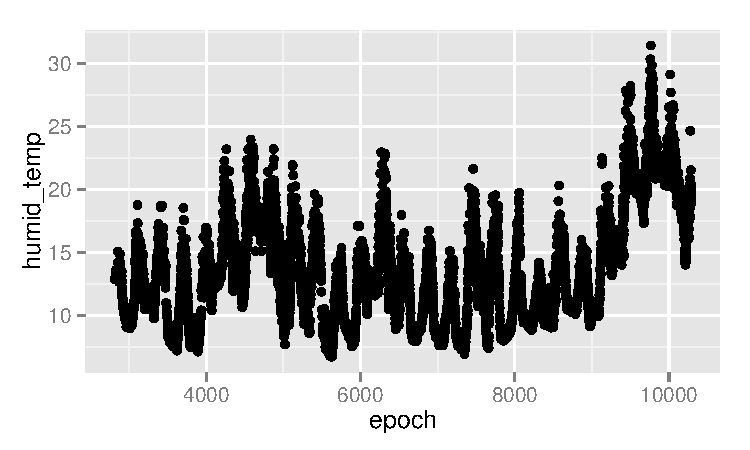
\includegraphics[width=\maxwidth]{figure/plot_cleansed_net_epoch_temperature} 

}

\caption[Cleansed temperature over time]{Cleansed temperature over time\label{fig:plot_cleansed_net_epoch_temperature}}
\end{figure}


\end{knitrout}

\ref{fig:plot_cleansed_net_epoch_humidity}
\begin{knitrout}
\definecolor{shadecolor}{rgb}{0.969, 0.969, 0.969}\color{fgcolor}\begin{figure}[h!]


{\centering 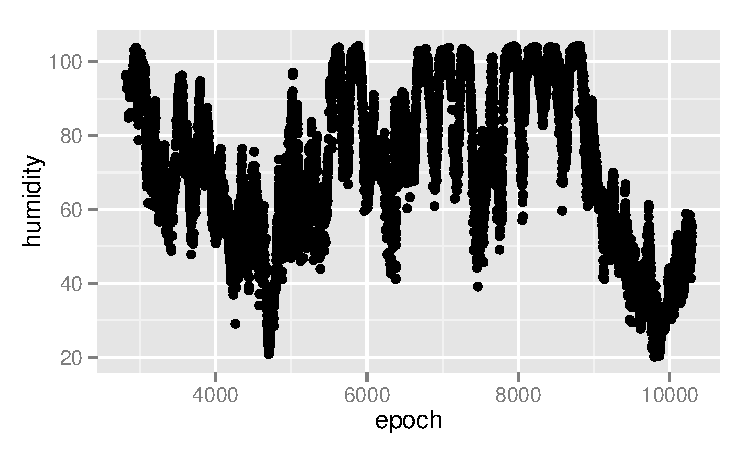
\includegraphics[width=\maxwidth]{figure/plot_cleansed_net_epoch_humidity} 

}

\caption[Cleansed humidity over time]{Cleansed humidity over time\label{fig:plot_cleansed_net_epoch_humidity}}
\end{figure}


\end{knitrout}


With sensible values, we can now anaylze whether these values make sense over time.  Several plots can reveal pattern outliers.



\end{document}
